%\documentclass[preprint,tightenlines,showpacs,showkeys,floatfix,
%nofootinbib,superscriptaddress,fleqn]{revtex4} 
\documentclass[floatfix,nofootinbib,superscriptaddress,fleqn,notitlepage]{revtex4-2}   
%\documentclass[aps,epsfig,tightlines,fleqn]{revtex4}
\usepackage{kotex}
\usepackage[HWP]{dhucs-interword}
\usepackage[dvips]{color}
\usepackage{graphicx}
\usepackage{bm}
%\usepackage{fancyhdr}
%\usepackage{dcolumn}
\usepackage{defcolor}
\usepackage{amsmath}
\usepackage{amsfonts}
\usepackage{amssymb}
\usepackage{amscd}
\usepackage{amsthm}
\usepackage[utf8]{inputenc}
%\pagestyle{fancy}
\usepackage{tikz}
\begin{document}

\title{\Large 2022년 2학기 물리학 II}
\author{김현철\footnote{Office: 5S-436D (면담시간 매주
    화요일-16:00$\sim$18:00)}} 
\email{hchkim@inha.ac.kr}
\author{Hui-Jae Lee} 
\email{hjlee6674@inha.edu}
\affiliation{Hadron Theory Group, Department of Physics,
  Inha  University, Incheon 22212, Republic of Korea }
\date{Autumn Semester, 2022}

\maketitle

{\color{red} {\bf Date:} 2022년 8월 29일  15:30-16:15 }
\vspace{1.cm}

\section*{\large Quiz 1}
\noindent {\bf 문제 1 [10pt]}
다음 질문에 답하세요.
\begin{itemize}
\item[(가)] 전하의 종류를 적으세요 (2pt). 
\item[(나)] 전하량을 유효숫자 두 자리까지 적으세요 (2pt). 
\item[(다)] 아래에 주어진 과정 중에서 틀린 과정을 고르세요 (2pt).
  \begin{enumerate}
  \item $e^++e^-\to \gamma + \gamma$
  \item $\pi^0 + p \to \pi^+ + n$
  \item $p+n\to p+p$
  \item $\Lambda^0\to p + e^- +\bar{\nu}_e$
  \end{enumerate}
\item[(라)] 쿨롱의 법칙을 식으로 나타내고 설명하세요 (4pt). 
\end{itemize}
\vspace{1.cm}

\noindent {\bf 풀이 : }
\begin{itemize}
  \item[(가)] 전하의 종류는 양전하와 음전하로 2가지 존재한다.
  \item[(나)] 전자 1개의 전하량을 유효숫자 두 자리가지 적으면 $1.6\times 10^{-19}~\mathrm{C}$이며 
  C는 전하량의 단위로 쿨롱이라 읽는다.
  \item[(다)] $e$는 전자, $\gamma$는 광자, $\pi$는 $\pi$ 중간자($\pi$ meson), 
  $p$와 $n$은 양성자, 중성자이며 $\Lambda$와 $\bar{\nu}_e$는 각각 $\Lambda$ 중입자
  ($\Lambda$ baryon)와 전자 반중성미자(electron antineutrino)이다.  \\
  전하량 보존 법칙에 따라 과정 전 전하의 총합과 과정 후 전하의 총합은 같아야 한다.
  \begin{enumerate}
    \item 과정 전 전하의 합은 $1+(-1)=0$이고 과정 후 전하의 합 또한 $0+0=0$이므로 
    전하량 보존 법칙에 비추어 보았을 때 과정은 틀리지 않았다.
    \item 과정 전 전하의 합은 $0+1=1$이고 과정 후 전하의 합은 $1+0=1$이므로
    전하량 보존 법칙에 비추어 보았을 때 과정은 틀리지 않았다.
    \item 과정 전 전하의 합은 $1+0=1$이고 과정 후 전하의 합은 $1+1=2$이므로
    전하량 보존 법칙에 비추어 보았을 때 과정은 틀렸다.
    \item 과정 전 전하의 합은 $0$이고 과정 후 전하의 합은 $1+(-1)+0=0$이므로
    전하량 보존 법칙에 비추어 보았을 때 과정은 틀리지 않았다.
    \end{enumerate}
    틀린 과정은 3번 과정이다.
  \item[(라)] 쿨롱의 법칙은 식으로 나타내면 다음과 같다.
  \begin{align}
    F=k\frac{q_1q_2}{r^2}.
  \end{align}
  이는 전하를 띈 두 입자 사이에 작용하는 힘의 크기에 대한 법칙으로 두 전하 사이에 작용하는 힘은 
  두 전하가 떨어진 거리의 제곱에 반비례함을 의미한다. $k$는 쿨롱 상수로 그 크기는
  $8.988\times 10^{9}~\mathrm{N\cdot m^2\cdot C^{-2}}$ 이다.
\end{itemize}

\vspace{1.cm}
\noindent {\bf 문제 2 [10pt]}
전자와 양성자가 대략 보어 반지름, 즉 $0.530\times 10^{-10}$ m 정도
떨어져 있다. 전자와 양성자 사이의 전기력과 중력을 각각 구하고, 구한
전기력과 중력의 비를 구하여라. 
\vspace{1.cm}

\noindent {\bf 풀이 : } 전자와 양성자의 전하량을 $q_1$, $q_2$라 하고 둘 사이 거리를 $r$이라 하자.
쿨롱의 법칙에 의해 전자와 양성자 사이 작용하는 전기력 $F_e$는
\begin{align}
  \begin{split}
    F_e &= k\frac{q_1q_2}{r^2} = (8.988\times 10^{9}~\mathrm{N\cdot m^2\cdot C^{-2}})
    \frac{(1.60\times 10^{-19}~\mathrm{C})(1.60\times 10^{-19}~\mathrm{C})}
    {(0.530\times 10^{-10}\mathrm{m})^2} \\
    &= 8.19\times 10^{-8}~\mathrm{N}
  \end{split}
\end{align}
이고, 전자와 양성자의 질량을 $m_1$, $m_2$라고 하면 전자와 양성자 사이 작용하는 중력 $F_g$는
\begin{align}
  \begin{split}
    F_g &= G\frac{m_1m_2}{r^2}=(6.67\times 10^{-11}~\mathrm{N\cdot m^2\cdot kg^{-2}})
    \frac{{(9.11\times 10^{-31}~\mathrm{kg})}
    {(1.67\times 10^{-27}~\mathrm{kg})}}{(0.530\times 10^{-10}\mathrm{m})^2}\\
    &=3.61\times 10^{-47}\mathrm{N}
  \end{split}
\end{align}
이다. 전자와 양성자 사이에 작용하는 두 힘의 비는 다음과 같다.
\begin{align}
  \frac{F_e}{F_g}=\frac{8.19\times 10^{-8}~\mathrm{N}}{3.61\times 10^{-47}\mathrm{N}}
  =2.27\times 10^{39}.
\end{align} 
전자와 양성자 사이 작용하는 전기력이 중력보다 무려 $10^{39}$배 만큼 크다.

\vspace{1.cm}
\noindent {\bf 문제 3 [10pt]}
일직선상에 세 점전하가 간격 $d$를 두고 놓여 있다. 전하량은 순서대로
$-q$, $+q$, $-q$이다. 각 전하에 작용하는 힘을 구하여라.
\vspace{1.cm}

\noindent {\bf 풀이 : }
가운데 놓여있는 점전하 $+q$를 원점으로 하고 오른쪽을 양의 방향으로 하자. 중첩의 원리에 의해 각 점전하가
받는 전기력은 나머지 두 점전하로부터 받는 전기력의 합과 같다. 
\begin{figure}[htp]
  \centering
  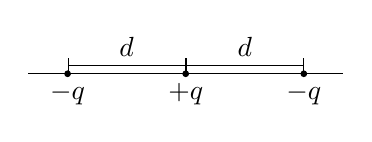
\begin{tikzpicture}
    \filldraw[black] (0,0) circle (1pt) node[anchor=north]{$+q$};
    \filldraw[black] (1.5,0) circle (1pt) node[anchor=north]{$-q$};
    \filldraw[black] (-1.5,0) circle (1pt) node[anchor=north]{$-q$};
    \draw (-2,0) -- (2,0) ;
    \draw[|-|] (0,0.1) -- node[above] {$d$} (1.5,0.1);
    \draw[|-|] (0,0.1) -- node[above] {$d$} (-1.5,0.1);
  \end{tikzpicture}
  \caption{일직선 위의 세 점전하}
  \label{fig:11}
\end{figure}
왼쪽에 있는 전하부터 순서대로 1, 2, 3번
전하라고 하겠다. 먼저 원점에 있는 2번 전하가 받는 힘을 구해보자. $\vec{F}_{ij}$는 $i$번 전하가 
$j$번 전하로부터 받는 전기력으로
\begin{align}
  \vec{F}_{ij}=k\frac{q_i q_j}{|\vec{r}_i-\vec{r}_j|^3}(\vec{r}_i-\vec{r}_j)
\end{align}
$2$번 전하가 받는 전기력 $\vec{F}_2$는
\begin{align}\label{eq:3-1}
  \vec{F}_2 = \vec{F}_{21}+\vec{F}_{23}
\end{align}
이다. 각각의 전하로부터 $d$만큼 떨어져 있으므로 각 힘을 계산하여
\begin{align}
  \vec{F}_{21}=k\frac{(+q)(-q)}{d^3}(0-(-d))\hat{x}=-\frac{kq^2}{d^2}\hat{x},\,\,\,
  \vec{F}_{23}=k\frac{(+q)(-q)}{d^3}(0-d)\hat{x}=\frac{kq^2}{d^2}\hat{x}
\end{align}
를 얻는다. 식~\ref{eq:3-1}에 대입하여 2번 입자에 작용하는 전기력을 구하면
\begin{align}
  \vec{F}_2 = -\frac{kq^2}{d^2}\hat{x}+\frac{kq^2}{d^2}\hat{x}=\vec{0}
\end{align}
이다. 작용과 반작용에 의하면 $i$번 전하가 $j$번 전하로부터 받는 전기력은 $j$번 전하가 $i$번 전하로부터 
받는 전기력과 크기는 같고 방향만 반대이다. 따라서
\begin{align}
  \vec{F}_{ij}=-\vec{F}_{ji}
\end{align} 
임을 알 수 있다. 이제 나머지 1번, 3번 점전하에 작용하는 전기력을 구해보자. 1번 전하에 작용하는 전기력 
$\vec{F}_1$은
\begin{align}
  \vec{F}_1 = \vec{F}_{12}+\vec{F}_{13} =-\vec{F}_{21}+\vec{F}_{13}
\end{align}
$\vec{F}_{13}$을 계산하면 구할 수 있다. 1번 전하와 3번 전하는 $2d$만큼 떨어져 있으므로
\begin{align}
  \vec{F}_{13} = k\frac{(-q)(-q)}{(2d)^3}((-d)-d)\hat{x}
  =-\frac{kq^2}{4d^2}\hat{x}
\end{align}
를 얻는다. 그러므로 $\vec{F}_{1}$은
\begin{align}
  \vec{F}_{1} = -\left(-\frac{kq^2}{d^2}\hat{x}\right)+\left(-\frac{kq^2}{4d^2}\hat{x}\right)
  =\frac{3kq^2}{4d^2}\hat{x}
\end{align}
를 얻는다. 같은 방법으로 $\vec{F}_{3}$은
\begin{align}
  \vec{F}_{3} = \vec{F}_{31}+\vec{F}_{32} = -\vec{F}_{13}-\vec{F}_{23}
\end{align}
이고 $\vec{F}_{13}$과 $\vec{F}_{23}$은 위에서 이미 구해 놓았다.
\begin{align}
  \vec{F}_{3} = -\left(-\frac{kq^2}{4d^2}\hat{x}\right)
  -\frac{kq^2}{d^2}\hat{x}=-\frac{3kq^2}{4d^2}\hat{x}.
\end{align}
$\vec{F}_{3}$과 $\vec{F}_{1}$은 크기는 같고 방향만 다르다.

\vspace{1.cm}
\noindent {\bf 문제 4 [10pt].} 
질량이 $m=3.00\times 10^{-2}$ kg이고 대전된 전하량이 같은 작은 공 두
개가 그림~\ref{fig:2}와 같이 길이가 $L=0.150$ cm인 줄에 매달려
있다. 각 $\theta$는 $5.00^\circ$이다. 
각각의 공에 대전된 전하량을 구하여라. 
\begin{figure}[htp]
  \centering
  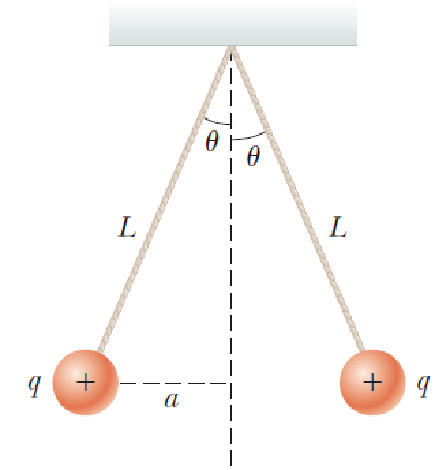
\includegraphics[scale=0.6]{Qfig20220827-2.pdf}
  \caption{\textbf{문제 4}}
  \label{fig:2}
\end{figure}
\vspace{1.cm}

\noindent {\bf 풀이 : } 먼저 정지해있는 왼쪽 공의 자유 물체 다이어그램을 그려보자. 공에 작용하는 장력을 
$T$, 중력을 $F_g$, 전기력을 $F_e$라고 하면 세 힘이 평형을 이루어 공이 정지해 있다고 생각할 수 있다. 
\begin{figure}[htbp]
  \centering
  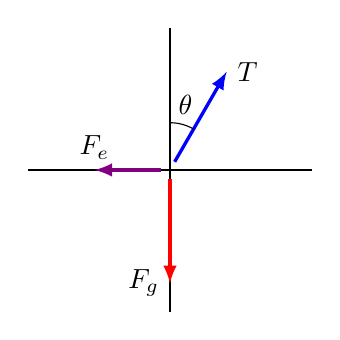
\begin{tikzpicture}[scale=1.2]
    \draw (0,-1.5) -- (0,1.5); 
    \draw (-1.5,0) -- (1.5,0);
    \draw[red,very thick,-latex] (0,-0.1) -- (0,-1.2) 
    node [left,black] {$F_g$};
    \draw[rotate=-30,blue,very thick,-latex] (0,0.1)--(0,1.2)
    node [above,black,right] {$T$};
    \draw[rotate=60] (0.5,0) arc(0:30:0.5) (0.5,0.1)
    node [above] {$\theta$};
    \draw[violet,very thick,-latex] (-0.1,0) -- (-0.8,0) 
    node [above,black] {$F_e$};
  \end{tikzpicture}\caption{왼쪽 공의 다이어그램}
\end{figure}

$x$방향과 $y$방향의 운동방정식을 다음과 같이 세울 수 있다. 공이 정지해 있으므로 모든 방향에서의 합력은
0이다.
\begin{align}
  F_x&= -F_e+T\sin\theta=0,\label{eq:4-1} \\
  F_y&= T\cos\theta-F_g=0.\label{eq:4-2}
\end{align}
먼저 $y$방향 합력으로부터 장력 $T$를 구하자. 공의 질량을 $m$이라 하면 $F_g=mg$이므로
\begin{align}\label{eq:4-3}
  F_g=mg\Longrightarrow mg-T\cos\theta=0,\,\,\,T=\frac{mg}{\cos\theta}
\end{align}
를 얻는다. 한편 공 두개가 대전된 전하량이 같으므로 쿨롱의 법칙에 의해 공에 작용하는 전기력 $F_e$는
\begin{align}
  F_e = k\frac{q^2}{(2a)^2}
\end{align}
인데 $a$는 줄의 길이 $L$의 삼각비로 표현할 수 있다.
\begin{align}\label{eq:4-4}
  a = L\sin\theta.
\end{align}
따라서 식~\ref{eq:4-1}에 식~\ref{eq:4-3}과 식~\ref{eq:4-4}를 대입하면
\begin{align}
  -k\frac{q^2}{(2L\sin\theta)^2}+mg\tan\theta=0
\end{align}
을 얻는다. 
$m=3.00\times 10^{-2}$ kg, $L=1.50\times 10^{-3}$ m이고 $\theta=5.00^\circ$이므로
전하량 $q$는
\begin{align}
  \begin{split}
    q &= 2L\sin\theta\sqrt{\frac{mg\tan\theta}{k}}
    =2(1.50\times 10^{-3}~\mathrm{m})\sin 5.00^\circ
    \sqrt{\frac{(3.00\times 10^{-2}~\mathrm{kg})(9.807~\mathrm{m/s^2})\tan 5.00^\circ}
    {(8.988\times 10^{9}~\mathrm{N\cdot m^2\cdot C^{-2}})}} \\
    &= 4.42\times 10^{-10}~\mathrm{C}
  \end{split}
\end{align}
임을 알 수 있다.

\vspace{1.cm}

\noindent {\bf 문제 5 [10pt].} 
질량이 $m$이고 전하 $q$로 대전된 두 부도체를 길이가 $L_0$이고 용수철
상수가 $k$인 용수철에 연결하였더니 용수철의 길이가 $4L_0/3$로 늘어나
평형상태가 되었다. 이제 두 대전된 부도체 중 하나를 $x=0$에 고정시키고
용수철에 연결된 또 다른 부도체가 단순조화운동을 하게 한다면, 각진동수
$\omega$는 $\sqrt{k/m}$의 몇 배인가? 
\vspace{1.cm}

\noindent {\bf 풀이 : }
평형상태의 부도체에 작용하는 힘에는 용수철에 의한 복원력과 부도체끼리 밀어내려는 전기력이 있다. 두 힘의 크기가
같아 평형상태를 이루므로 훅의 법칙과 쿨롱의 법칙을 이용하여
\begin{align}\label{eq:5-1}
  \sum F = -k\frac{1}{3}L_0+\frac{1}{4\pi\epsilon_0}
  \frac{q^2}{\left(\frac{4}{3}L_0\right)^2}=0\Longrightarrow
  k\frac{1}{3}L_0=\frac{1}{4\pi\epsilon_0}\frac{q^2}{\left(\frac{4}{3}L_0\right)^2},\,\,\,
  k=\frac{q^2}{4\pi\epsilon_0}\frac{27}{16L_0^3}
\end{align}
를 얻는다. 평형상태에 있는 부도체를 단순조화운동시키기 위해 길이 $x_0$만큼 잡아당겼다고 가정하자. 이 때
용수철의 길이는 $\frac{4}{3}L_0+x_0$가 되고 용수철의 길이가 $\frac{4}{3}L_0$일 때
새로운 평형이 이루어진 것이므로 늘어난 길이는 $x_0$가 된다. 늘어난 길이에서의 전기력과
용수철의 복원력을 고려하여 훅의 법칙을 다시 쓰면
\begin{align}\label{eq:5-2}
  \sum F = ma = -k\left(\frac{1}{3}L_0+x_0\right)+\frac{1}{4\pi\epsilon_0}\frac{q^2}
  {\left(\frac{4}{3}L_0+x_0\right)^2}
\end{align} 
이다. 잡아당긴 길이 $x_0$가 $L_0$에 비해 무시할 수 있을만큼 작다고
가정하면, 즉, $x_0/L_0<<1$이라고 하면 우변의 마지막 항을 근사할 수 있다.
\begin{align}\label{eq:5-3}
\frac{1}{(1+\epsilon)^2}\approx 1-2\epsilon\Longrightarrow
\frac{1}{\left(\frac{4}{3}L_0+x_0\right)^2}=\frac{9}{16L_0^2}
\frac{1}{\left(1+\frac{3x_0}{4L_0}\right)^2}\approx
\frac{9}{16L_0^2}\left(1-\frac{3x_0}{2L_0}\right).
\end{align}
이 결과와 식~\ref{eq:5-1}를 식~\ref{eq:5-2}에 대입하여 다시쓰면
\begin{align}
  \begin{split}
    ma&=-k\left(\frac{1}{3}L_0+x_0\right)+\frac{q^2}{4\pi\epsilon_0}
    \frac{9}{16L_0^2}\left(1-\frac{3x_0}{2L_0}\right)
    =-k\left(\frac{1}{3}L_0+x_0\right)+kL_0\frac{1}{3}\left(1-\frac{3x_0}{2L_0}\right)\\
    &=-k\left(\frac{1}{3}L_0+x_0\right)+k\left(\frac{1}{3}L_0-\frac{1}{2}x_0\right)
    =-k\frac{3}{2}x_0
  \end{split}
\end{align}
이다. 따라서 각진동수 $\omega$는
\begin{align}
  \omega=\sqrt{\frac{3}{2}}\sqrt{\frac{k}{m}}
\end{align}
으로 $\sqrt{k/m}$의 $\sqrt{3/2}$배이다. 즉, 전기력이 없을 때에 비해 약 1.22배 빠르게 진동한다.
\vspace{1.cm}

\end{document}